\let\negmedspace\undefined
\let\negthickspace\undefined
\documentclass[journal]{IEEEtran}
\usepackage[a5paper, margin=10mm, onecolumn]{geometry}
%\usepackage{lmodern} % Ensure lmodern is loaded for pdflatex
\usepackage{tfrupee} % Include tfrupee package

\setlength{\headheight}{1cm} % Set the height of the header box
\setlength{\headsep}{0mm}     % Set the distance between the header box and the top of the text

\usepackage{gvv-book}
\usepackage{gvv}
\usepackage{cite}
\usepackage{amsmath,amssymb,amsfonts,amsthm}
\usepackage{algorithmic}
\usepackage{graphicx}
\usepackage{textcomp}
\usepackage{xcolor}
\usepackage{txfonts}
\usepackage{listings}
\usepackage{enumitem}
\usepackage{mathtools}
\usepackage{gensymb}
\usepackage{comment}
\usepackage[breaklinks=true]{hyperref}
\usepackage{tkz-euclide} 
\usepackage{listings}
% \usepackage{gvv}                                        
\def\inputGnumericTable{}                                 
\usepackage[latin1]{inputenc}                                
\usepackage{color}                                            
\usepackage{array}                                            
\usepackage{longtable}                                       
\usepackage{calc}                                             
\usepackage{multirow}                                         
\usepackage{hhline}                                           
\usepackage{ifthen}                                           
\usepackage{lscape}
\begin{document}

\bibliographystyle{IEEEtran}
\vspace{3cm}

\title{9-9.2-43}
\author{AI24BTECH11022 - Pabbuleti Venkata Charan Teja}
\maketitle

\renewcommand{\thefigure}{\theenumi}
\renewcommand{\thetable}{\theenumi}

\textbf{Question:}

Find the area of the region bounded by the curve $y=x^{2}$ and $y=x+6$ and $x=0$.\\

\textbf{Solution:}

\begin{table}[h!]
\renewcommand{\thetable}{1}
    \centering
   \begin{tabular}{|c| c |}
\hline
\textbf{Variable} & \textbf{Value} \\
\hline
$A$ & \myvec{1 \\ -5\\}\\
\hline
$B$ & \myvec{-4 \\ 5\\}\\
\hline
$k:1$    & Ratio in which the line $AB$ is divided by $x$-axis \\
\hline
$X$  & Point of division of $A$ , $B$\\
\hline
\end{tabular} 
   \def\tablename{Table}
   \caption{Variables Used}
    \label{tab9.9.2.43.1}
\end{table}

The given curve can be expresssed as a conic with parameters 
\begin{align}
    V=\myvec{1 & 0\\ 0 & 0\\},u=\myvec{0 \\ \frac{-1}{2}\\},f=0
\end{align}


The given line parameters are 
\begin{align}
    h=\myvec{-6 \\ 0\\},m=\myvec{1 \\ 1\\}
\end{align}


Substituting from the above in $$k_{i}=\frac{1}{m^{\top}Vm}\brak{-m^{\top}\brak{Vh+u}\pm\sqrt{\sbrak{m^{\top}\brak{Vh+u}}^{2}-g\brak{h}\brak{m^{\top}Vm}}}$$ gives 
\begin{align}
    k_{1}=4,k_{2}=9
\end{align}

Substituting values of $k_{i}$ in $x_{i}=h+k_{i}m$ gives points of intersection of the line and the curve 
\begin{align}
    \implies x_{1}=\myvec{-2 \\ 4\\},x_{2}=\myvec{3\\ 9\\}
\end{align}

According to the plot,

The required area in 2nd Quadrant is 
\begin{align}
    Area&=\int_{-2}^{0}\brak{x+6}-x^{2}dx\\
    Area&=\frac{22}{3}
\end{align}


The required area in 1st Quadrant is 
\begin{align}
    Area&=\int_{0}^{3}\brak{x+6}-x^{2}dx\\
    Area&=\frac{27}{2}
\end{align}


\begin{figure}[h!]
\renewcommand{\thefigure}{1}
    \centering
    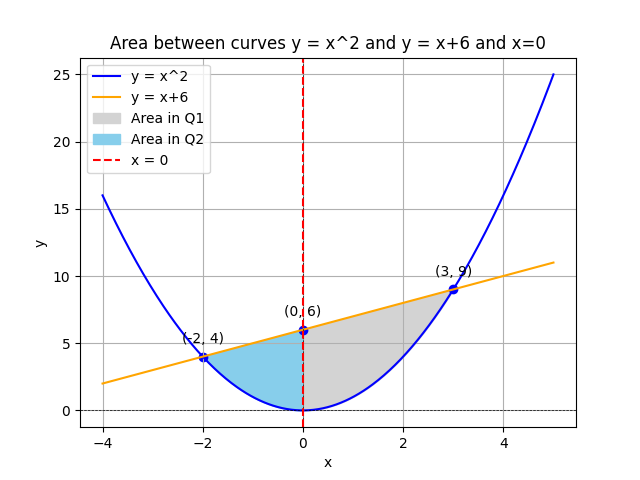
\includegraphics[width=0.7\linewidth]{figs/plot.png}
    \caption{Plot of the points}
    \label{fig9.9.2.43.1}
\end{figure}

\end{document}
